\section{Non-parametric Localization}
So far, we have seen localization based on parametric filtering techniques. Now we will look at utilizing
some of the non-parametric filtering techniques discussed earlier to formulate non-parametric localization.
The following two subsections discuss Grid Localization and Monte Carlo Localization.

\subsection{Grid Localization}
Grid localization is a variant of the discrete Bayes filter and is mainly based on the principles of histogram filtering. The main idea is to approximate the posterior belief using a histogram filter over the grid decomposition of the state space:

$$ dom(X_t) = x_{1,t}\cup x_{2,t}\cup...x_{K,t} $$

Hence, at time $t$, the state space is partitioned into $K$ grids. Following this, the posterior is represented as a collection of discrete probability values:

$$ bel(x_t) = \{p_{k,t}\}$$

where $p_{k,t}$ represents the probability of belonging to grid cell $k$ at time $t$. Similar to the histogram filter, the motion and measurement models are also discretized with an additional conditioning on the map $m$. The pseudocode in Figure 13.1 follows the same pattern as earlier localization methods. The input consists of the belief at time $t-1$, the control action $u_t$, the measurement $z_t$, and the map $m$ of the environment. The algorithm outputs the updated belief at time $t$.

The algorithm has a prediction step where the predicted belief $\{\Bar{p}_{k,t}\}$ is calculated using a total probability theorem as shown in the algorithm. The total probability theorem uses the probability belief calculated for each cell $i$ at time $t-1$ defined as $p_{i,t-1}$ and the probability of reaching cell $k$ and the map $m$. The last step normalizes the probability using the factor $\eta$, which is computed along with the probability belief $p_{k,t}$.

%% Including graphics
\begin{center}
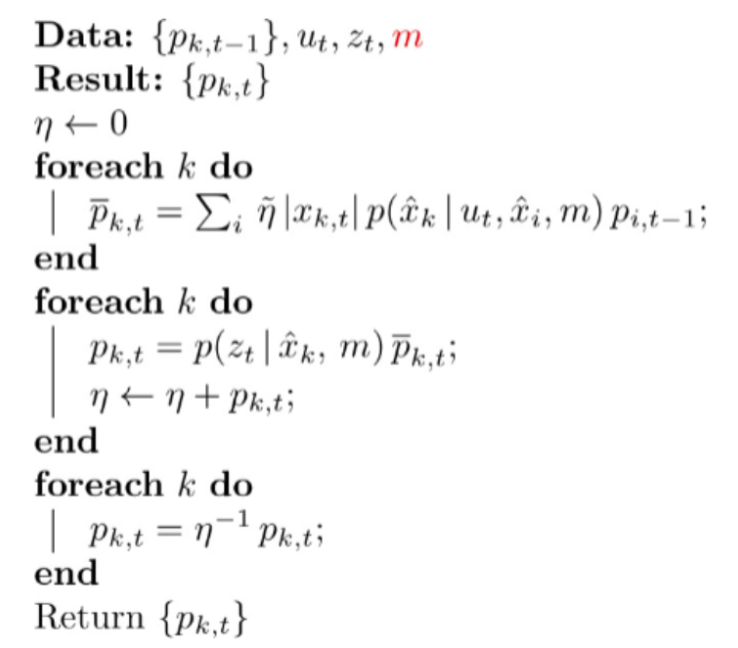
\includegraphics[scale = 0.5]{gridLocalization.png}\\
Figure 13.1: Pseudocode for Grid Localization
\end{center}

To decompose the state space into a discrete set of cells, there are multiple methods. One possible choice is topological, where decomposition is based on significant spaces. Another method is a uniform decomposition of state space into cells of equal size. Grid localization has a trade-off between retaining information from the continuous state space and complexity of computation. As the system uses more grids with higher resolution, the computational complexity increases. Some of the techniques used to reduce the computation complexity are pre-caching, sensor subsampling, delayed motion updates and selective updating.

\subsection{Monte Carlo Localization}
%%%%% I have started this section
Monte Carlo Localization is a localization algorithm that follows from the particle filtering technique. For this algorithm, the belief at time $t$ is defined as:
$$ bel(x_t) = \chi = \{x_t^{[1]}, x_t^{[2]}, \ldots , x_t^{[M]}\} $$

where $x_t^{[i]}$ is the i-th particle at time $t$. As in grid localization, the input consists of the control action $u_t$, the measurement $z_t$, and the map m of the environment along with the belief at time $t-1$. The output is a new set of particles representing the belief at time $t$.

During the prediction step, M particles $\{x_{t}^{[m]}\}_{m=1}^M$
are sampled. Precisely, the particle $x_t^{[i]}$ is sampled from
the motion model conditioned on the current particle $x_{t-1}^{[m]}$
and the control action $u_t$. A weight $w_t^{[m]}$ is assigned to each particle which indicates the confidence in that particle. This weight is calculated from the measurement model conditioned on the measurement $z_t$, the sampled particle $x_t^{[m]}$
and the map $m$. 
The predicted belief $\bar{\chi_t}$ is a set containing tuples of particles and their associated weights. Then, in order to update $\chi_t$, the algorithm randomly samples $M$ particles with a probability distribution based on the confidence weights. So a particle with a higher weight could appear multiple times in the updated set $\chi_t$, whereas a particle with a weight set to 0 would never appear. Thus, through this predicting and updating process, the belief narrows down to a set of particles with a high level of confidence. The pseudo-code for the algorithm is shown in Figure 13.2.

%% Including graphics
\begin{center}
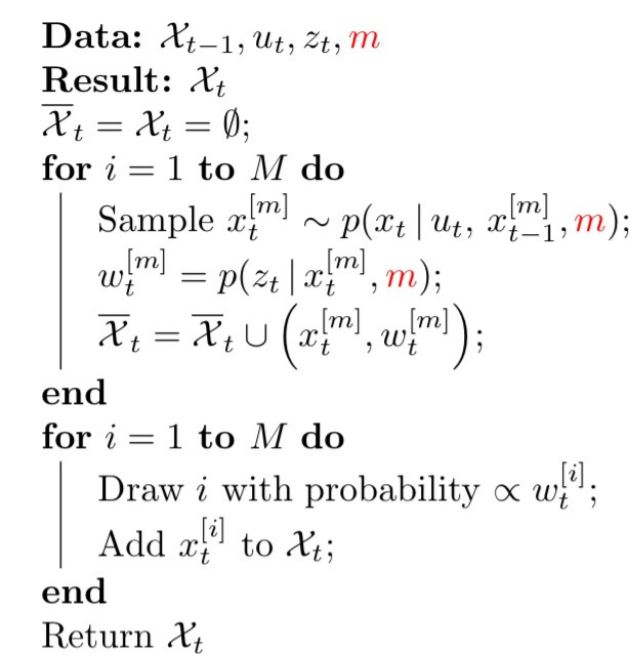
\includegraphics[scale = 0.5]{MonteCarlo.JPG}\\
Figure 13.2: Pseudocode for Monte Carlo Localization [1]
\end{center}

Figure 13.3 provides an illustration of the Monte Carlo Localization algorithm. At the beginning, the robot is unaware of its location and the particles (black dots) are spread out widely in block (a). As the updating of particles progresses in block (b), the robot is able to narrow down its belief on its position to fewer regions shown by the clusters of particles. Eventually, the robot is very confident about its position as
shown by the single cluster of particles in block (c). This algorithm can address some cases such as global localization, robot kidnapping, position tracking, and dynamic environments.

%% Including graphics
\begin{center}
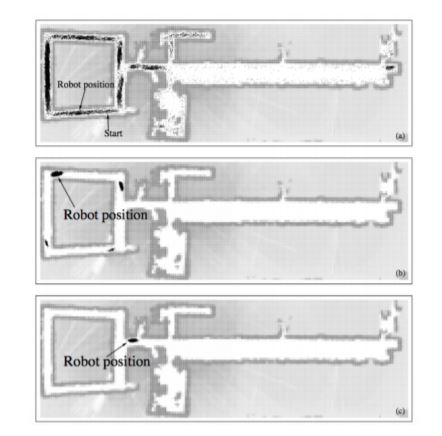
\includegraphics[scale = 0.5]{monte_illustration.JPG}\\
Figure 13.3: Illustration of Monte Carlo Localization [1]
\end{center}

%% Including graphics
\begin{center}
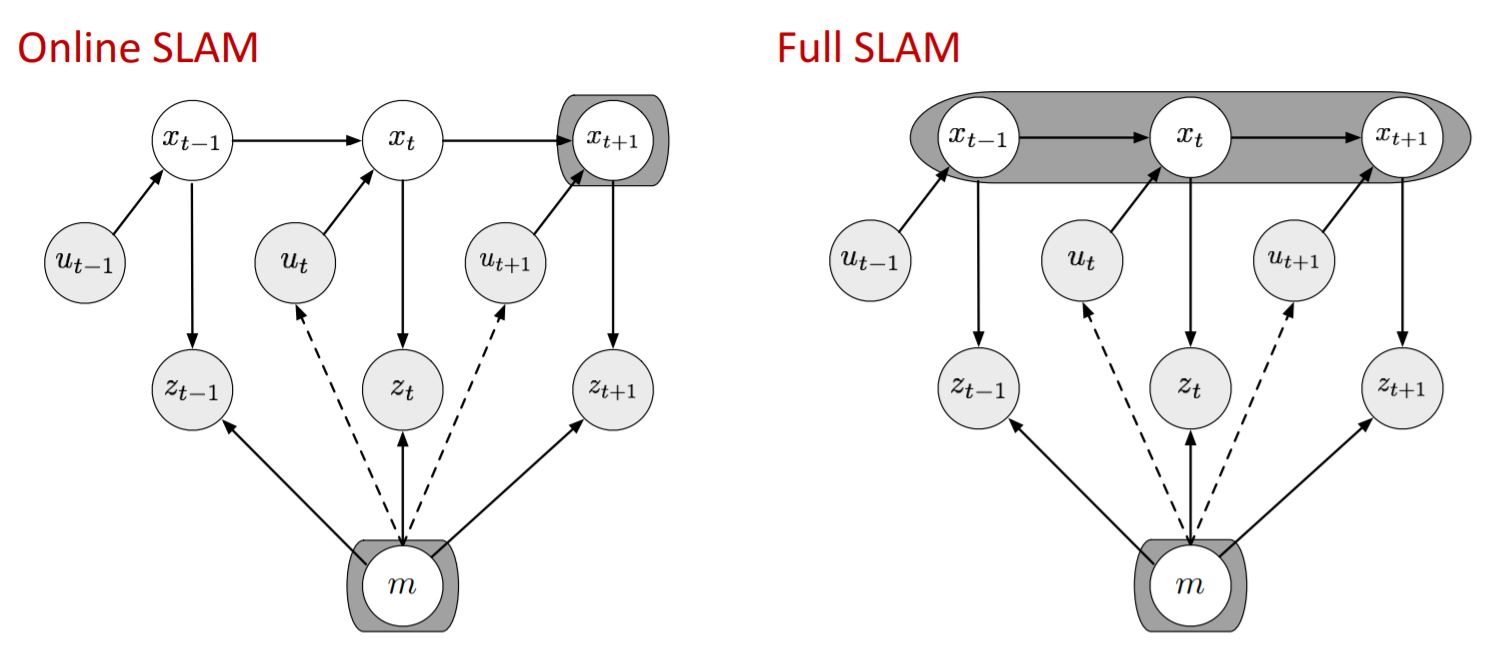
\includegraphics[scale = 0.4]{SLAM_Difference.JPG}\\
Figure 13.4: Difference between online and full SLAM
\end{center}
